
% W tym rozdziale Autor opisze skrótowo zadania które wykonywały badane modele sieci, oraz zaprezentuje wyniki badań - czyli czasy realizacji zadania przez zbudowane modele.

\section{ Zadanie 1 - regresia liniowa }
Zadanie zaczerpnięto z \cite{Osowski2023} i polegało na wyznaczeniu czasu obliczeniu funkcji polyfit:

\begin{equation*}
p(x)=p_1 x^n +p_2x^{n−1} + ... + p_nx + p_{n+1}
\end{equation*}

Dane wejściowe wygenerowano losowo i zapisano w pliku. Użyto tych samych danych we wszystkich realizacjach. W językach C++ i Java napisano własny kod:


\begin{center}
\begin{tabular}{ |c|c| } 
 \hline
 
 C++ & Python \\

 \hline

    \begin{lstlisting}[language=c++,numbers=none,basicstyle=\tiny,frame=none]
for (int c = 0; c < CYCLES; c++) {
   xsr = 0.0; ysr = 0.0; 
   w1  = 0.0; w0  = 0.0;
   for ( int i=0; i<len; i++ ){
      xsr +=  X[i];
      ysr +=  Y[i];
   }
   xsr=xsr / len;
   ysr=ysr / len;

   double sumTop=0.0;
   double sumBottom=0.0;
   for ( int i=0;i<len;i++ ){
      sumTop   += ((X[i]-xsr)*(Y[i]-ysr));
      sumBottom += ((X[i]-xsr)*(X[i]-xsr));
   }
   w1 = sumTop / sumBottom;
   w0 = ysr -(w1 * xsr) ;
}
    \end{lstlisting}
 & 

\begin{lstlisting}[language=c++,numbers=none,basicstyle=\tiny,frame=none]
for ( int C=0; C<cycles; C++ ) {
   double xsr = 0.0;
   double ysr = 0.0;
   for (int i = 0; i < x.length; i++) {
      xsr += x[i];
      ysr += y[i];
   }
   xsr = xsr / x.length;
   ysr = ysr / y.length;

   w1 = 0.0;
   w0 = 0.0;
   double sumTop = 0.0;
   double sumBottom = 0.0;
   for (int i = 0; i < x.length; i++) {
      sumTop += ((x[i] - xsr) * (y[i] - ysr));
      sumBottom += ((x[i] - xsr) * (x[i] - xsr));
   }
   w1 = sumTop / sumBottom;
   w0 = ysr - w1 * xsr;
}
    \end{lstlisting}
 
 \\

 \hline 
\end{tabular}
\end{center}





W językach Python i Matlab wykorzystano dostępne funkcje języka:


\begin{center}
\begin{tabular}{ |c|c| } 
 \hline
 
 Matlab & Python \\

 \hline

    \begin{lstlisting}[language=c++,numbers=none,basicstyle=\small,frame=none]
for i = 1:cycles
    a = polyfit(x,y,1);    
end
    \end{lstlisting}
 & 

\begin{lstlisting}[language=c++,numbers=none,basicstyle=\small,frame=none]
for c in range( cycles ):
    a = np.polyfit(x,y,1)

    \end{lstlisting}
 
 \\

 \hline 
\end{tabular}
\end{center}

\newpage
Zadanie realizowano bez użycia GPU, czas wczytania danych jest pomijany.

\begin{figure}[ht]
    	\centering 
            \includegraphics[width=0.95\linewidth]{rysunki/fig01.jpg} 
            \caption{Zadanie 1 - zestawienie czasu obliczeń w zależności od liczby próbek w serii, skala logarytmiczna }
\end{figure} 
W kolejnych seriach wielkość zbioru zwiększano o 10. Odnotowano, że przy dużych zbiorach danych program w C++ naruszał ochronę pamięci, a system kończył jego pracę, (i zgłaszając błąd). \newline
Zestawienie ogólnej wydajności języków w kolejności od najszybszego wygląda następująco:
\begin{enumerate}
  \item C++
  \item Java     
  \item Matlab
  \item Python
\end{enumerate}  


\newpage
\section{ Zadanie 2 - perceptron wielowarstwowy }
*** CHECK ***

Struktury głębokich sieci neuronowych, takich jak LaNet, AlexNet i inne, mogą różnić się ilością i rodzajem warstw. Istnieje jednak struktura pojawiająca się na wyjściu z sieci prawdopodobnie we wszystkich rozwiązaniach. Strukturą tą jest perceptron wielowarstwowy MLP, na schematach sieci jej warstwy opisane są "Fully-Connected" lub skrótem "FC". Warstwy ukryte perceptronu mogą mieć dowolne funkcje aktywacji: funkcje logistyczną, ReLU lub podobną do ReLU. Jeśli sieć realizuje zadanie klasyfikacji wieloklasowej, wtedy ostatnia wyjściowa warstwa perceptronu jest warstwą Softmax.
Głęboka sieć splotowa pracuje na trójwymiarowych strukturach danych zwanych tensorami, perceptron wielowarstwowy przetwarza jednowymiarowe struktury danych. Aby była możliwa współpraca sieci głębokiej i perceptronu wielowarstwowego, potrzebna jest warstwa spłaszczająca, której zadaniem jest konwersja tensora do wektora podczas wnioskowania, i konwersja wektora do tensora w procesie uczenia. 
%%
*** /CHECK ***
%%
To zadanie również zaczerpnięto z \cite{Osowski2023}. Polegało ono na zbudowaniu modelu sieci MLP, a następnie przeprowadzeniu procesu uczenia sieci klasyfikującej cyfry pisanych ręcznie. Założono wykonanie 100 epok uczenia przy wykorzystaniu 50\% objętości zbioru danych uczących.
%%
Zaproponowano sieć MLP o strukturze :
%%
\begin{itemize}
    \item Warstwa 1: 64 perceptronów, wejścia 784, aktywacja - funkcja sigmoidalna
    \item Warstwa 2: 64 perceptronów, wejścia~ 64, aktywacja - funkcja sigmoidalna
    \item Warstwa 3: 10 perceptronów, wejścia~ 64, aktywacja - funkcja softmax
\end{itemize}
%%
\begin{figure}[ht]
    	\centering 
            \includegraphics[width=0.65\linewidth]{rysunki/mnist_prev.jpg} 
\end{figure} 
%%
W procesie wykorzystano zestaw obrazów treningowych i testowych ze zbiorów MNIST \cite{zestawDanychMNIST}\newline
%%
%%
W Matlabie wykorzystano dostępne dodatki, a w Pythonie zainstalowano biblioteki Scikit-learn, zaś w kolejnym rozwiązaniu Tensorflow.
%%
\begin{center}
\begin{tabular}{ |c|c| } 
 \hline

 Matlab & Python Scikit-learn \\

 \hline

    \begin{lstlisting}[language=c++,numbers=none,basicstyle=\footnotesize ,frame=none]
    
neurons=64;
net = feedforwardnet([64,64],'traingd'); 
net.trainParam.epochs = 100;
net.trainParam.goal   = 0.0003;
net.input.processFcns = {'mapminmax'};
net.output.processFcns = {'mapminmax'};

gxtrain = gpuArray( xtrain );
gytrain = gpuArray( ytrain );

net = configure(net,xtrain,ytrain);
net = train(net, gxtrain, gytrain, \
    'useParallel','yes','useGPU','yes');
    \end{lstlisting}
 & 

\begin{lstlisting}[language=c++,numbers=none,basicstyle=\footnotesize ,frame=none]

net = snn.MLPClassifier( \
   hidden_layer_sizes=(64,64), \
   max_iter=100, \
   random_state=1, \
   alpha=0.0001, \
   early_stopping=False, \
   activation='logistic', \
   solver='sgd', \
   learning_rate='constant', \
   learning_rate_init=0.001 )

start=time.time()
net.fit( trainX, trainY )
    \end{lstlisting}
 
 \\

 \hline 
\end{tabular}
\end{center}
\begin{figure}[ht]
    	\centering 
            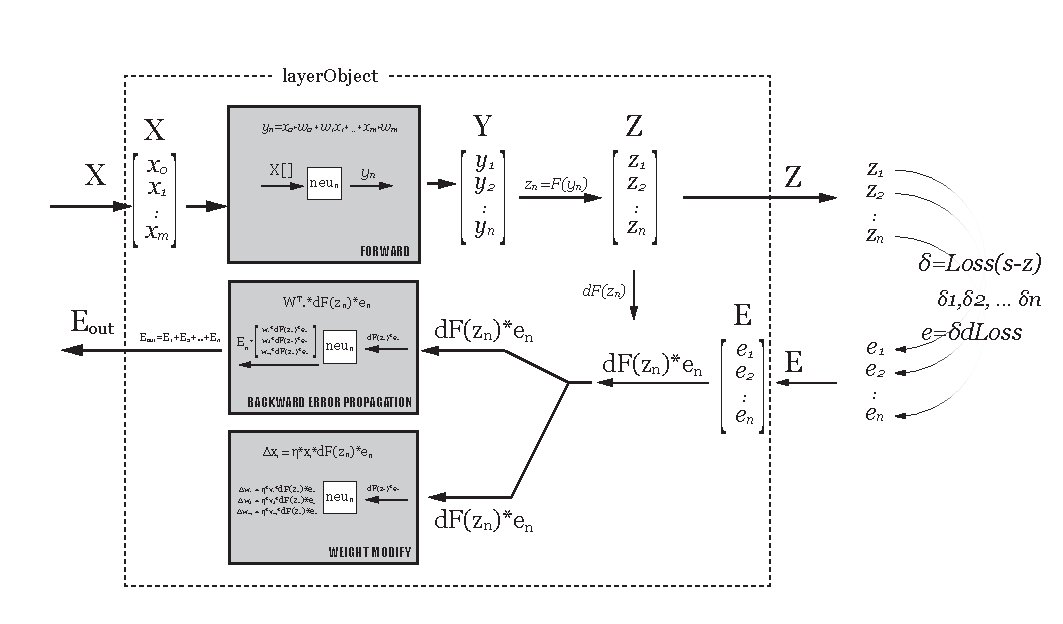
\includegraphics[width=0.74\linewidth]{rysunki/rys1_4.jpg} 
\end{figure} \newpage
Rozwiązanie w Javie oparto na własnej implementacji sieci MLP. Szczególny nacisk położono na czytelność kodu i idei kosztem wydajności. Wykorzystano wiedzę z poprzednich rozdziałów i napisano kod zgodnie z zasadami programowania obiektowego. Zasady hermetyzacji wymuszają utworzenie dwu współpracujących ze sobą obiektów: neurosumatora oraz warstwy. Własnością warstwy jest rodzaj funkcji aktywacji, a jej metodą jest obliczenie pochodnej funkcji aktywacji w punkcie pracy.
%%
%%
\begin{figure}[ht]
    	\centering 
            \includegraphics[width=0.72\linewidth]{rysunki/zad2.jpg} 
            \caption{Zadanie 2 - zestawienie czasów uczenia perceptronu MLP }
\end{figure} 
%%
\begin{figure}[ht]
    	\centering 
            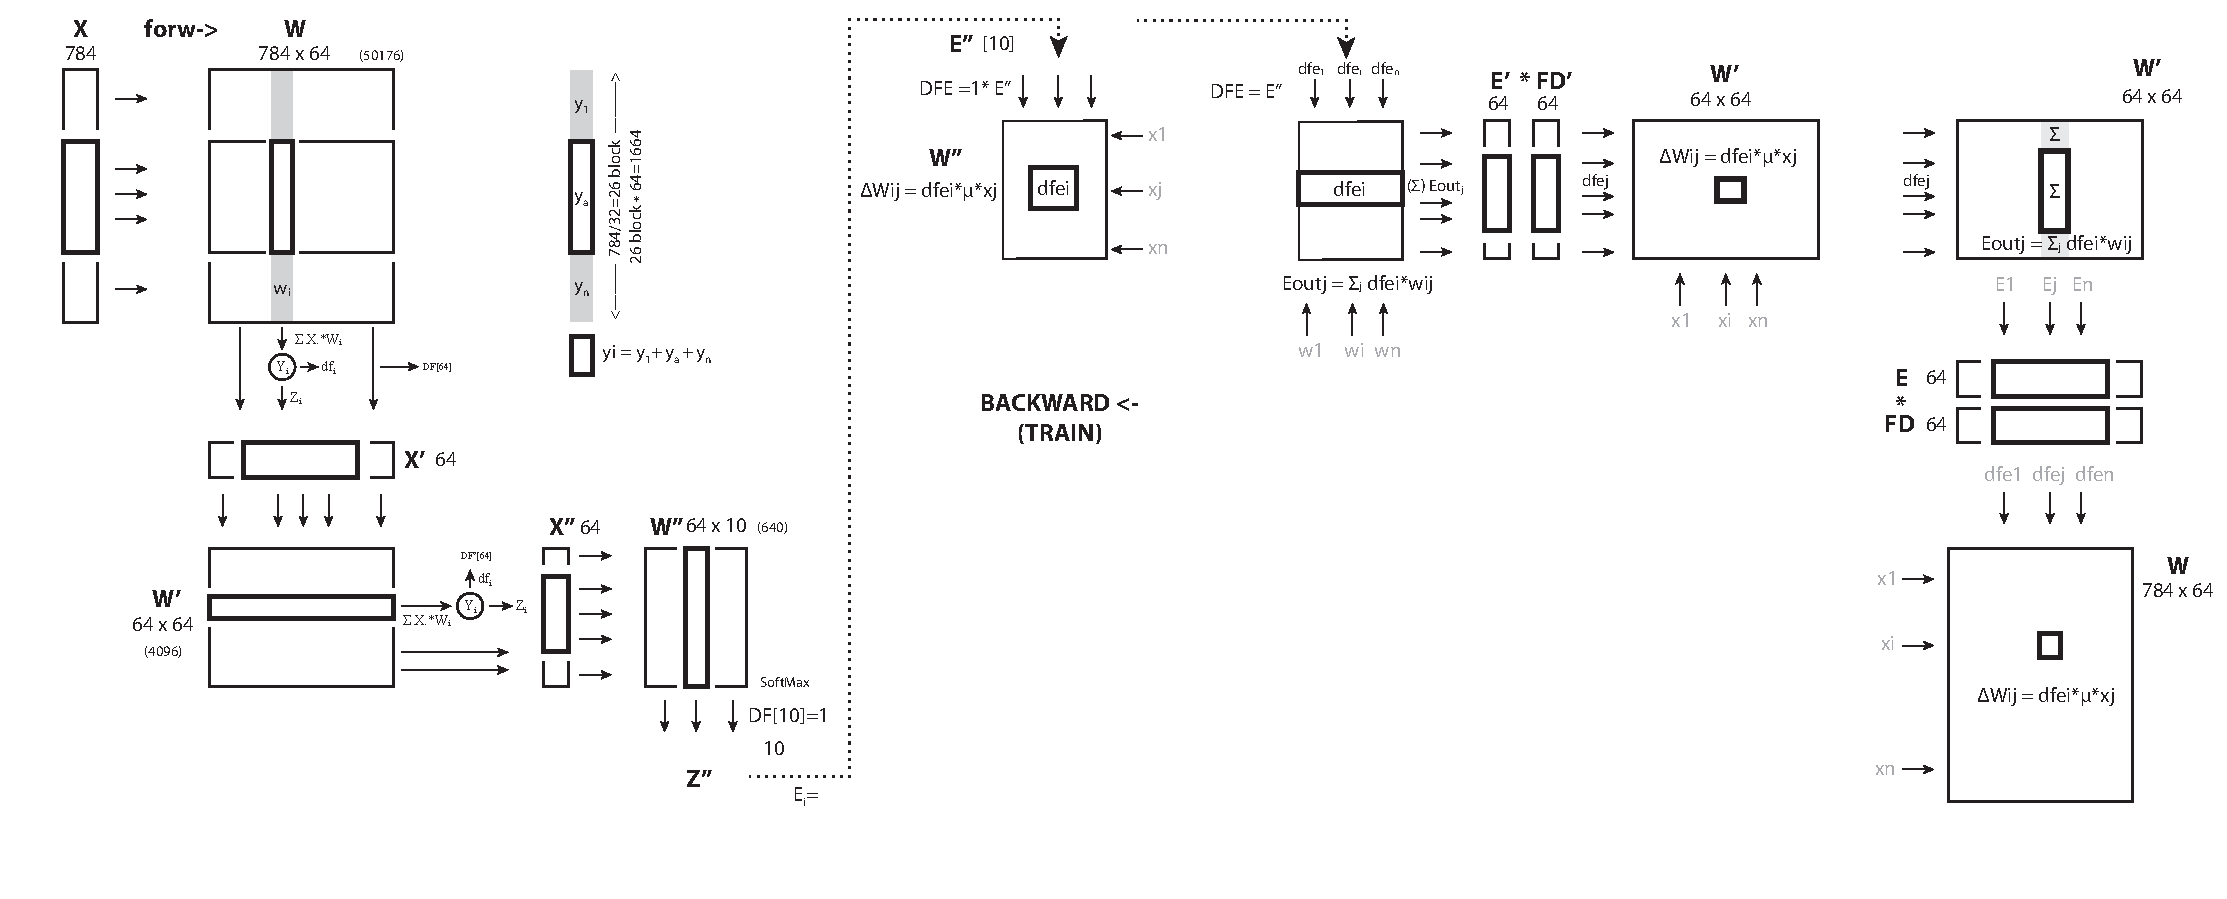
\includegraphics[width=0.72\linewidth]{rysunki/CUDA_train_process.jpg} 
            \caption{Zadanie 2 - obliczenia na GPU}
\end{figure}
%%
\begin{figure}[ht]
    	\centering 
            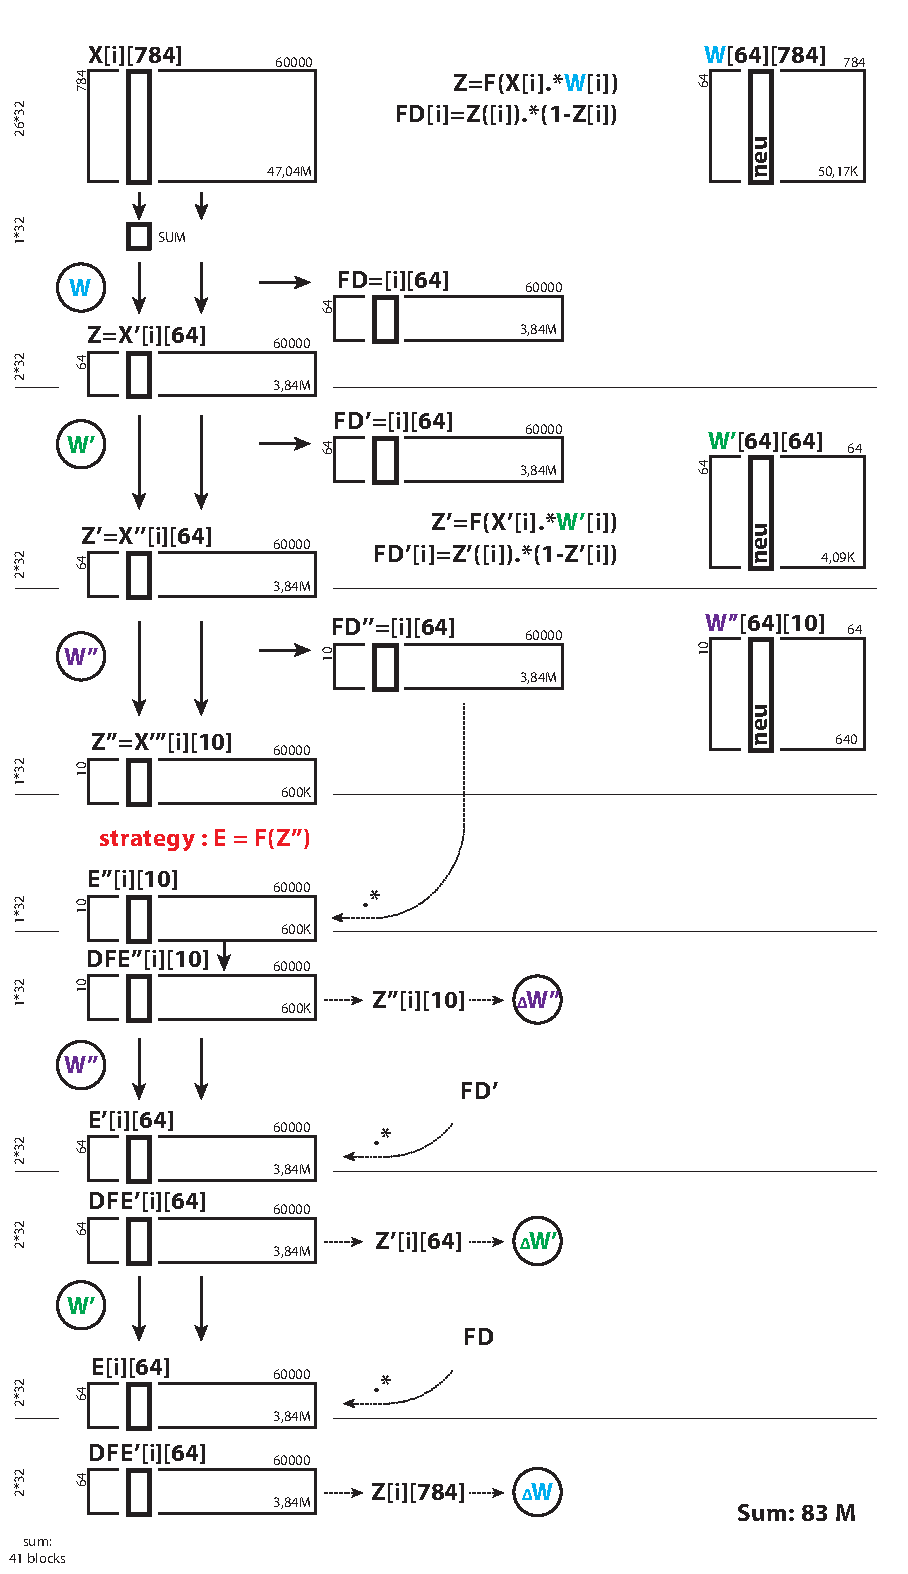
\includegraphics[width=0.42\linewidth]{rysunki/CUDA_memory.jpg} 
            \caption{Zadanie 2 - obliczenia na GPU mapa pamięci}
\end{figure}
%%
\section{ Zadanie 3 - sieć splotowa }
Zadanie polegało na zbudowaniu modelu sieci splotowej CNN połączonej z siecią MLP, wg. struktury LaNet-5 zaproponowanej przez prof. Yann LeCun \cite{YannCnn}  przedstawionej m.in. w \cite{Osowski2023}.
%%
%%
Przeprowadzeniu procesu uczenia sieci, polegającego na rozpoznawaniu cyfr pisanych ręcznie. Założono wykonanie 100 epok uczenia, przy wykorzystaniu 100\% objętości zbioru danych uczących.
%%
Struktura sieci:
\begin{itemize}
    \item Warstwa 1: Wejście obraz 28x28 pikseli 1 kanał.
    \item Warstwa 2: Konwolucyjna, 20 @ filtr 5x5, aktywacja ReLU.
    \item Warstwa 3: Normalizacja
    \item Warstwa 4: PoolMax, rozmiar 2x2, krok 2x2
    \item Warstwa 5: Spłaszczenie obrazu do jednowymiarowej tablicy
    \item Warstwa 6: MLP: 64 neurony, aktywacja ReLU
    \item Warstwa 7: MLP: 10 neuronów, wyjście Softmax
\end{itemize} 
%%
%%
\begin{center}
%%
\begin{tabular}{ |c|c| }  \hline
 Python PyTorch & Python Tensorflow.Keras \\
 \hline
    \begin{lstlisting}[language=c++,numbers=none,basicstyle=\tiny ,frame=none]
\\ CITE -> https://www.datacamp.com/
\\       tutorial/pytorch-cnn-tutorial
\\ Javier Canales Luna

class CNN(nn.Module):
def __init__(self, in_channels, num_classes):
    super(CNN, self).__init__()
    self.conv1 = nn.Conv2d(in_channels=in_channels, \
    out_channels=20, kernel_size=5, padding=1)
    self.norm  = nn.BatchNorm2d(20)
    self.pool = nn.MaxPool2d(kernel_size=2, stride=2)
    self.fc1 = nn.Linear( 3380, 64 )
    self.fc2 = nn.Linear( 64, num_classes )

def forward(self, x):
    x = F.relu(self.conv1(x))
    x = self.norm(x)
    x = self.pool(x)
    x = x.reshape(x.shape[0], -1)
    x = self.fc1(x)
    x = self.fc2(x)
    return x

start=time.time()
for epoch in range(epochs):
   scores = model(data)
   loss = criterion(scores, targets)
   optimizer.zero_grad()
   loss.backward()
   optimizer.step()
    \end{lstlisting}
    
 & 

\begin{lstlisting}[language=c++,numbers=none,basicstyle=\tiny ,frame=none]
\\ CITE -> https://keras.io/examples/
\\              vision/mnist_convnet/

 def AlexNet():
   NUMBER_OF_CLASSES = 10
   return keras.models.Sequential([
      keras.layers.Input(shape=( 28, 28, 1 )),
      keras.layers.Conv2D(name='conv1', \
      filters=20, kernel_size=(5,5), \
      activation='relu' ),
      keras.layers.BatchNormalization(),
      keras.layers.MaxPool2D(pool_size=(2,2), \
      strides=(2,2)),
      keras.layers.Flatten(),
      keras.layers.Dense(64, activation='relu'),
      keras.layers.Dense(10, activation='softmax')
])
model = AlexNet()
model.compile(optimizer='adam',
  loss='sparse_categorical_crossentropy',
  metrics=['accuracy'])
start=time.time()

with tf.device('/device:GPU:0'):
   model.fit(trainX, trainY, epochs=epochs, verbose=0)

    \end{lstlisting}
 
 \\

 \hline 
\end{tabular}
\end{center}
\newpage
W zadaniu wykorzystano dane z zadania 2, Dwa rozwiązania zostały napisane w Pythonie z wykorzystaniem bibliotek PyTorch oraz Tensorflow. Jedno rozwiązanie powstało w Matlabie z wykorzystaniem bibliotek systemowych. W języku Java napisano własne rozwiązanie, w którym przyjęto te same założenia i strukturę jak w zadaniu 2, rozszerzono działanie klas w projekcie tak by realizowały sieć splotową CNN oraz działanie warstw pomocniczych, ReLU, Flatten, Max i Avg.
%%
\begin{figure}[ht]
    	\centering 
            \includegraphics[width=0.72\linewidth]{rysunki/zad3.jpg} 
            \caption{Zadanie 3 - zestawienie czasów uczenia sieci CNN }
\end{figure} \newpage














\newpage
\section{ Zadanie 4 - głęboka sieć splotowa }
Zadanie polegało na zbudowaniu modelu głębokiej sieci splotowej CNN i nauczeniu sieci rozpoznawania twarzy. Przygotowany zbiór zdjęć uczących i testowych pochodził z zasobów publicznych internetu. 
~ \newline
\begin{figure}[ht]
    	\centering 
            \includegraphics[width=0.8\linewidth]{rysunki/zad4.jpg} 
            \caption{ Zadanie 4 - zestawienie czasów uczenia sieci głębokiej CNN }
\end{figure} 
~ \newline
\begin{figure}[ht]
    	\centering 
            \includegraphics[width=0.95\linewidth]{rysunki/zad4.jpg} 
\end{figure} 
\newline 
Rozwiązanie zrealizowano w dwu językach: Matlab i Python Tensorflow. 







\section{ Zadanie 5 - widzenie komputerowe }
Zadanie polegało na zbudowaniu aplikacji Yolo8 w językach Python i C++, z wykorzystaniem nauczonego modelu dostarczonych przez ultralytics. Oceniono czas wykonania rozpoznawania obiektów na obrazie. Porównania dokonano tak jak w poprzednich przypadkach w środowisku wyposażonym w kartę graficzną, a następnie powtórzono w tym samym środowisku już bez karty.

~ \newline
\begin{figure}[ht]
    	\centering 
            \includegraphics[width=0.8\linewidth]{rysunki/zad5.jpg} 
            \caption{ Zadanie 4 - zestawienie czasów rozpoznawania obiektów Yolo8 }
\end{figure} 